% Kailash Ranganathan
% Spring 2023
% kranganathan@berkeley.edu
% Edited by Dun-Ming Huang, dunmingbrandonhuang@berkeley.edu

\qns{Comparators and their Applications}

\textbf{Learning Goal:} This problem will give intuition for how comparators function and also how to design more complex circuits with comparators. Hopefully, you'll also learn the basics of how analog-to-digital converters work too!


\begin{enumerate}
    \item {
        Using an op-amp, a $V_{ref} = 3V$ voltage reference, a  a $5V$ voltage source, and a reference to ground,\textbf{ construct a comparator whose output is governed by the following characteristics:}
        \begin{equation}
            V_{out} = 
                \begin{cases}
                    5 & \text{if } V_{in} > 1.5V\\
                    0 & \text{if } V_{in} < 1.5V \\
                \end{cases}
        \end{equation}
        Don't worry about the case where $V_{in} = 1.5V$, and assume you also have an unlimited supply of $1 k\Omega$ resistors. \emph{Hint: think about how you can exploit railing in open-loop op amps to give you comparator-like behavior.}
    }
    \ans{
        Before thinking about the comparator, lets think about the hint and what would happen for op-amp railing. \\
        Suppose we had an op-amp with a very high gain (effectively infinity). Then, if $u_+ > u_-$ by only a very small amount, we may observe that
        \[
            V_{out} = A (u_+ - u_-) >> 1
        \]
        the output voltage will become very high as though $(u_+ - u_-)$ is small, multiplying by a near-infinite number will give an extremely high output. Of course, the op-amp does not have an infinite power supply, so it can only give voltage values up to $V_{DD}$. \\ \\ 
        We can somewhat start seeing the pattern here. If $u_+ < u_-$ (even if only by a little bit), $V_{out} = A(u_+ - u_-) << -1$, the output voltage will become very negative. The op-amp does not have an infinite \textit{negative} power supply either, so it will \textbf{rail} at $V_{SS}$, meaning that it is unable to supply output any lower. \\ \\ 
        \textbf{Thus, an ideal op-amp in open-loop (ie. with its terminals not connected in any way) resembles comparator behavior with finite terminal railing! If $u_+ > u_-$, then $V_{out} = V_{DD}$, and likewise if $u_+ < u_-$, then $V_{out} = V_{SS}$.} \\ \\
        Now, we can apply these concepts to the specifications given in the problem. We can pattern-match $V_{in}$ to $u_+$ and $1.5V$ to $u_-$, likewise pattern matching $V_{DD}$ to $5V$ and $V_{SS}$ to $0V$. \\ \\ 
        To get the $1.5V$ value at $u_-$, note that we don't actually have a $1.5V$ voltage source. Instead, we'll have to use a voltage divider with $3V$ and equal resistors (if this doesn't make sense, think about what resistors you'd need in a voltage divider to get "half" of a $3V$ source). We only have $1 k\Omega$ resistors, so the easiest voltage divider is with 2 of these. If this all sounds abstract, a circuit diagram is provided below of what the op-amp comparator should look like. 

        \begin{center}
            \begin{circuitikz}[transform shape]
    	\draw
            
    	(0,0) node[op amp] (AMP) {}
            (0, -0.5) to[short, -o] ++(0, -1)
                node[below]{$V_{DD}$}
            (0, 0.5) to[short] ++(0, 1)
                node[ground,rotate=180]{}
    	(AMP.-) to[short] ++(-2,0) coordinate (intersect)
    		to[R,l_=$1k\Omega$] ++(-2,0)
    		to[V_=$3V$] ++(0,-2)
    		node[ground]{}
    	(intersect) to[R,l_=$1k\Omega$] ++(0,-2) node[ground]{}
    	(AMP.+) to[short] ++(-1, 0) 
                to[sV^=$V_{in}$] ++(0, -1.5)
                node[ground]{}
            (AMP.out) to[short, -o] ++(1, 0)
                node[right]{$V_{out}$}
            ; 
            \end{circuitikz}
        \end{center}

        The op-amp diagram is vertically flipped which is why $V_{DD}$ is on the bottom and ground is on the top, but observe that they still act as the positive and negative rails respectively. Also note that $V_{in}$ is on the \textit{positive} input of the op-amp whereas the fixed $1.5V$ is on the negative input. 
    
    }

    \item {
        Draw the voltage plot of the above device (ie. plot $V_{out}$ by $V_{in}$ (you may assume the op-amp is ideal -- that is, you may assume infinite gain). \\
    }
    \meta{
        For answering this question, it's sufficient to simply graph the step-function given in part a), but more importantly, students should understand how the op-amp replicates this behavior. Also, for 16A, any behavior where $u_+ = u_-$ is out-of-scope, so it's alright to say the op-amp (or comparator) behavior is undetermined at this point. 
        
    }
    \ans{
        The voltage plot is given by the piecewise $V_{out}$ function in the problem description (this is straightforward, but it's somewhat subtle to notice that this statement is only true \textit{because} the op-amp gain is infinite and so railing will immediately happen when $u_+$ crosses above or below $u_-$). 
    
        \begin{center}
            \begin{tikzpicture}
                \begin{axis}[
                    axis lines = left, 
                    xlabel = \(V_{in}\),
                    ylabel = {\(V_{out}\)},
                    title = {Graph of Comparator Output: $V_{out}$ over $V_{in}$},
                    extra y ticks = {0}
                ]
                    \addplot[color=blue, ultra thick, domain=0:1.5, samples = 200]{0};
                    \addplot[color=blue, ultra thick, domain=1.5:5, samples = 200]{5};
                \end{axis}
            \end{tikzpicture}
        \end{center}
    }

    \item {
        Now, suppose the gain of the op-amp was finite; let's say $A = 2$. Draw the new voltage plot of the imperfect device (plot $V_{out}$ by $V_{in}$). For what range of $V_{in}$ values does the new op-amp not conform to the ideal characteristic (where we assume $A = \infty$)? \\
        \emph{Hint: think about the formula for op-amp output; exploring when the op-amp does/doesn't rail may be a good start.}
    }

    \ans{
        First, lets intuitively think about what would happen if the op-amp gain was finite (and not just finite, but pretty low, such as $A=2$). \\
        Then, immediately when $u_+ > u_-$, or $V_{in} > 1.5$, the op-amp output may not be high enough to rail instantly (which is what our initial configuration depended on). Rather, it will gradually increase to a certain point after which it'll reach the rail voltage $= V_{DD} = 5$, and then after that it will work as intended. \\
        Specifically, lets write out the op-amp $V_{out}$ equation explicitly.
        \begin{align*}
            V_{out} = A(u_+ - u_-) = 2(V_{in} - 1.5) = 2 V_{in} - 3
        \end{align*}
        This is just a linear relationship between input and output voltage, but with railing, we get the comparator-esque nonlinearity. Specifically, when $V_{out} < V_{SS} = 0V$, $V_{out}$ will constantly emit $0V$. This occurs when $2(V_{in} - 1.5) < 0$ (alternatively, $V_{in} < 1.5$). \\
        Thus, the part of our original comparator graph where $V_{out} = 0V$ is unchanged. \\ \\
        However, lets now see when our comparator rails on the positive end. For this, we need $V_{out} > 5V$, in which case $V_{out}$ will be clipped at $5V$. This occurs when $V_{out} = 2 V_{in} - 3 > 5 \xrightarrow{} V_{in} > 4$. Thus, positive railing doesn't start immediately once $V_{in} > 1.5V$, but rather it takes a while for the op-amp to reach this output voltage due to finite gain. \\ \\ 
        What happens in the middle of this range for $1.5 < V_{in} < 4V$? Here, $V_{out} = 2(V_{in} - 1.5)$ exactly as no positive or negative railing occurs, so we get a linear graph to connect the two ideal comparator outputs. The graph of this new piecewise function is shown below. 
    
        \begin{center}
            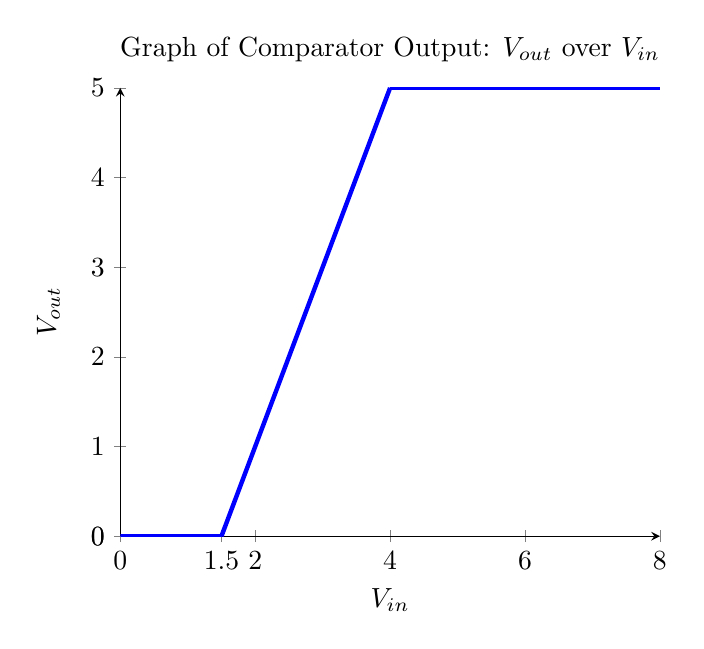
\begin{tikzpicture}
                \begin{axis}[axis lines = left, 
                xlabel = \(V_{in}\),
                ylabel = {\(V_{out}\)},
                title = {Graph of Comparator Output: $V_{out}$ over $V_{in}$},
                xtick = {0, 1.5, 2, 4, 6, 8},
                extra y ticks = {0}
                ]
                    \addplot[color=blue, ultra thick, domain=0:1.5, samples = 200]{0};
                    \addplot[color=blue, ultra thick, domain=1.5:4, samples=200]{2*(x-1.5)};
                    \addplot[color=blue, ultra thick, domain=4:8, samples = 200]{5};
                \end{axis}
            \end{tikzpicture}
        \end{center}
        Note how because of op-amp non-idealities, we lose the desired behavior of the "comparator" model for a certain range of $V_{in}$. 

    
    }
\end{enumerate}
\textbf{Digital to Analog Conversion} \\ 
    Comparators are very useful for a variety of applications, but one extremely significant application of comparators is in analog-to-digital conversion, a cornerstone of electrical engineering and circuit design. You'll learn the specifics of how it works in 16B -- for now, we just want to build up a rough idea of the ADC workflow. 
    \begin{center}
        \includegraphics[scale=0.5]{../../topics/op_amps/q_comparator_dac_figs/adc_circuit.png}
    \end{center}

    Consider the above diagram--we have some input analog signal $V_{in}$ connected to one terminal of a comparator. On the other terminal, we have the output voltage from a microcontroller (think of this controller as a black box for now), and the output of the comparator feeds back into the microcontroller. One ADC algorithm is to have the microcontroller continually "guess" what $V_{in}$ is, and use the feedback from the comparator to continually refine its guess. \\
    \textbf{Note that the "CMP1" circuit element is just a comparator (assume it's railed at $V_{DD} = 5V$ and $V_{SS} = 0V$).} 

\begin{enumerate}[resume]
    \item Given the following "guess voltages" $V_g$ coming from the microcontroller, provide the respective comparator output. Assume $V_{in} = 2.5V$. \
    \\ 
    \begin{center}
        \begin{tabular}{||c c c c||} 
         \hline
         $V_g$ out of P1 & CMP1 Output \\ [0.5ex] 
         \hline
         \hline
         5 &  \\ 
         \hline
         3.75 &   \\
         \hline
         2.4 &   \\
         \hline
         1.25 &  \\
         \hline
         0 &   \\ [1ex] 
         \hline
        \end{tabular}
    \end{center}

    \ans{
        Here, the behavior at different $V_g$'s is simply a matter of noticing what the behavior of CMP1 is. Remember the fundamental comparator rule; if $V_+ > V_-$, CMP1's output is $V_{DD} = 5V$. Else, CMP1's output is $V_{SS} = 0V$. Now, lets just notice what $V_+$ is and what $V_-$ is. In our circuit, $V_+ = V_{in}$ and $V_- = V_g$. We know $V_{in} = 2.5V$, so our CMP1 output will just be $5V$ whenever $V_g < 2.5V$ and $0V$ whenever $V_g > 2.5V$. Thus, our output is as follows. 

        \begin{center}
        \begin{tabular}{||c c c c||} 
         \hline
         $V_g$ out of P1 & CMP1 Output \\ [0.5ex] 
         \hline\hline
         5 & 0 \\ 
         \hline
         3.75 & 0  \\
         \hline
         2.4 &  5 \\
         \hline
         1.25 & 5 \\
         \hline
         0 & 5  \\ [1ex] 
         \hline
        \end{tabular}
        \end{center}

        
    }

    \meta{ 
    Though unrelated to comparators, an interesting meta discussion if people are interested (and time permitting) would be to discuss how the algorithm works. Though we use binary search in 16B, you can think of just a linear search staritng at the maximum voltage and going down as our guesser. Immediately when our output from CMP1 goes from low to high, that last guess $V_g$ is our best approximation of $V_{in}$. This also explains why more bits means more resolution and thus a more accurate DAC conversion (so the shift from $0$ to $5V$ for comparator output will be as close to the actual $V_{in}$. This is an optional aside though, as the main purpose of this question is gaining practice with comparators and their application. 
    }
\end{enumerate}
    One last issue is that if $V_{in} > V_{max}$, our algorithm will not work (can you think of why?). We want to modify our circuit to look like the following to account for input "overflow." 
    \begin{center}
        \includegraphics[scale=0.8]{../../topics/op_amps/q_comparator_dac_figs/actual_adc_circuit_with_overflow.png}
    \end{center}
    Here, the microcontroller will take in a "control" input which, if digital high $= V_{DD}$, uses internal logic to bypass the DAC algorithm and prevent undesired behavior. \\ 
\begin{enumerate}[resume]
    \item {
        [CHALLENGE] Using a comparator, design a circuit in the block above such that:
        \begin{bindenum}
            \item If $V_{in} > V_{max}$, then $V_{DD} = 5V$ is sent to the control input of the microcontroller and $0V$ is sent to the rest of the ADC circuit.
            \item If $V_{in}$ is within the range, however, then $0V$ should be sent to the control input and the normal $V_{in}$ signal should be sent to the ADC circuit. 
        \end{bindenum}
        
    }

    \meta{This last question may be very tricky, especially figuring out how to exploit railing to get desired behavior. If students are struggling, it may be better to pose the alternative question to \textit{only} send either $0V$ or $5V$ to the control input and not worry about what goes into $V_{in}$}. 

    \ans{
    A possible design to the overflow control circuit is given in the following diagram: 
    \begin{center}
        \includegraphics[scale=0.4]{../../topics/op_amps/q_comparator_dac_figs/adc_circuit_overflow_solution.png}
    \end{center}


    This circuit is somewhat complicated/unintuitive, so lets first figure out what functionality we need our overflow control circuit to have, then figure out circuitry for each of those functions, and then build them up to get the above circuit. \\
    When designing a large, multi-feature circuit, we want to split our design into handling each feature separately, such that subsequent parts of the circuit can "abstract away" the details of previous parts and function as if they're always receiving normal input. 
    \begin{enumerate}
        \item \textbf{Overflow circuit logic:} Suppose $V_{in}$ enters from the left and is greater than $V_{DD}$. Then, we want the EN (control input) of the microcontroller to go high (aka to become $V_{DD}$). Thus, our first comparator will compare the value of $V_{in}$ to $V_{DD}$ and output its positive rail if $V_{in} > V_{DD}$ and its negative rail otherwise. Here, we make $V_{DD}$ not only an input into the comparator but \textit{also} its positive rail--when the input voltage is too high, it'll output $V_{DD}$ to the enable pin. If the input voltage is lower than our maximum, then the comparator just outputs ground and the DAC circuit proceeds normally. 
        \item \textbf{Input into DAC comparator} Now that we have the circuitry for the microcontroller enable pin done, we need to address what goes into the DAC according to problem specifications. If $V_{in}$ is outside of the maximum voltage, we should have $0V$ go to the rest of the circuit (so as to not potentially overload anything). We can do this by sending the output of our overflow comparator into another comparator, and compare it with some value in between $V_{DD}$ and $0V$ (hence the voltage divider). This value can be arbitrary, as long as it's a non-zero voltage below $V_{DD}$. Then, this comparator will output its positive rail if the overflow comparator output is high (ie. if $V_{in}$ is outside the allowed range) and its negative rail otherwise. Hence, we connect the negative rail to $V_{in}$ and the positive rail to ground. When the enable pin is high, this comparator will output $0V$ to the DAC circuit, and when the enable pin is low, the comparator will output $V_{in}$ to the DAC circuit for normal operation 
        \item \textbf{DAC comparator circuit} We don't actually need to change any part of this circuit as the previous circuit components have done the regulation for us. We can be guaranteed that we'll either receive a $V_{in}$ signal that's within the allowed range or we'll receive $0V$, in which case the enable pin being high will allow the microcontroller to do some internal error-handling logic. This reveals a very important lesson on abstraction for circuit design (yes, abstraction is useful not just in CS but EE too!). 
    \end{enumerate}


    }
    
\end{enumerate}
